\documentclass[12pt, openany]{report}
\usepackage[utf8]{inputenc}
\usepackage[T1]{fontenc}
\usepackage[french]{babel}
\usepackage{xcolor}
\usepackage{amsmath}
\usepackage[colorinlistoftodos]{todonotes}
\usepackage[colorlinks=true, allcolors=black]{hyperref}
\usepackage[a4paper,left=2cm,right=2cm,top=2cm,bottom=2cm]{geometry}
\usepackage{verbatim}
\usepackage{listings}
\usepackage{hyperref}
\usepackage{boxedminipage}
\usepackage{pgfgantt}
\usepackage{float}
\usepackage{pdfpages}
\usetikzlibrary{babel}
\usepackage{varioref}
\usepackage{listingsutf8}
\usepackage{algorithm2e}
\usepackage{libertine}

\bibliographystyle{alpha}


\setlength{\parindent}{0cm}
\setlength{\parskip}{1ex plus 0.5ex minus 0.2ex}
\newcommand{\hsp}{\hspace{20pt}}
\newcommand{\HRule}{\rule{\linewidth}{0.5mm}}

\renewcommand{\thesection}{\arabic{section}}

\begin{document}

\begin{titlepage}
  \begin{sffamily}
  \begin{center}

    \textsc{\LARGE Projet de programmation}\\[0.3cm]
    
    
\includegraphics[scale=0.35]{images/img2.jpg}~\\[0.8cm]

    % Title
    \HRule \\[0.4cm]
    { \huge \bfseries Génération de playlistes musicales pour un groupe d’utilisateurs\\[0.4cm] }
    
    \HRule \\[1.5cm]
    
\includegraphics[scale=0.4]{images/img1.png}
    \\[1.5cm]

    % Authors and supervisors
    \begin{minipage}{0.4\textwidth}
      \begin{flushleft} \large
        Legendre \textsc{Alexandre}\\
        Chauveau \textsc{Amandine}\\
        Berardet \textsc{Titouan}\\
        Chen \textsc{Zhong Yi}\\
        Martin--Delozanne \textsc{Delphine}\\
      \end{flushleft}
    \end{minipage}
    \begin{minipage}{0.4\textwidth}
      \begin{flushright} \large
        \emph{Responsable de l'UE : } M. \textsc{Philippe Narbel}\\
        \emph{Client : } M. \textsc{Pierre Hanna}\\
        \emph{Chargé de TD : } M. \textsc{Adrien Boussicault}
      \end{flushright}
    \end{minipage}

    \vfill

    % Bottom of the page
    {\large Version 1 : Janvier 2020 — Avril 2020}

  \end{center}
  \end{sffamily}
\end{titlepage}

\tableofcontents
\newpage

\section{Introduction}

Actuellement, tout utilisateur d'un service de streaming de musique, qu'il soit issu de Spotify ou de Deezer, peut se voir recommander des playlists en fonction de ses propres goûts musicaux.
Il peut arriver, cependant, que plusieurs utilisateurs veuillent écouter de la musique au même endroit. 
\\
\\
On se propose donc de répondre et de palier au schéma actuel, qui consiste à ce qu'une personne impose sa playlist à d'autres personnes.
On peut donc se poser la question suivante :
Qu'en est-il lorsqu'il s'agit de partager, entre plusieurs utilisateurs, une playlist globale qui puisse satisfaire ce même groupe d'utilisateurs ?
\\
\\
Notre projet consiste donc à proposer une alternative. 
Celle-ci se révélera par le développement d'une application mobile capable de générer cette playlist, satisfaisant les utilisateurs concernés par ce cas de figure.
Cette application devra inclure et respecter l'ensemble des besoins énoncés par le client, et devra être exemplaire en terme de fonctionnalités afin de permettre une utilisation correcte par les utilisateurs.

\section{Description et analyse de l'existant}

\subsection{Logiciels similaires}

\subsubsection{Flytrap : recommandation intelligente de musique pour un groupe}

Flytrap \cite {Flytrap} est un environnement musical qui se base sur les goûts de ses utilisateurs afin de  créer automatiquement une bande sonore qui peut plaire à toutes les personnes présentes dans une même pièce. Pour ce faire Flytrap regarde quelles sont les musiques que les utilisateurs écoutent et enregistre les pistes ainsi que des informations sur la musique dans une base de données. Le système utilise ensuite ces données et les combine avec la connaissance de la façon dont les genres de musique interagissent  entre eux pour prendre des décisions sur ce qu’un groupe d’utilisateurs pourrait vouloir écouter. \\
Afin de décider quelles pistes ajouter à une playlist, le système utilise un mécanisme de vote par lequel un «agent» représentant chaque utilisateur présent dans la salle donne un vote numérique à chaque piste dans la base de données du système. Si l’utilisateur a déjà écouté une musique de l’artiste ou si le genre est similaire à la musique qu’il écoute habituellement, la chanson reçoit un score élevé. Les musiques obtenant des scores plus élevés ont ainsi une plus forte probabilité d’être jouées. De plus, le système dispose également d’un agent de DJ qui priorise le résultat du vote de l’utilisateur en fonction de certaines règles : ne pas jouer deux musiques d’affilées du même artiste et maintenir une cohérence entre les genres. Flytrap gère donc intelligemment la musique dans un espace peuplé de gens aux goûts disparates en permettant de découvrir de nouvelles musiques d’artistes jamais écoutés mais ayant des qualités similaires aux musiques aimées par les utilisateurs.

\subsubsection{MusicFX}

MusicFX \cite {MusicFX} est un système de recommandation musicale qui permet aux membres d’un centre de fitness travaillant au même moment, d’influencer sans contrôler la musique diffusée.
\\
Pour ce faire, le système se base sur un algorithme qui prend en entrée un tableau représentant les préférences des utilisateurs présents dans la salle en fonction de genres musicaux. Ces valeurs vont de -2 (l’utilisateur déteste ce genre de musiques) à 2 (l’utilisateur adore ce genre de musiques). Une formule convertit alors toutes les préférences individuelles en des nombres non négatifs afin de pouvoir appliquer un opérateur de sélection aléatoire pondéré. Ces valeurs sont ensuite mises au carré afin d’élargir l’écart des probabilités de sélection entre les catégories les plus populaires et les catégories moins populaires. 
\\
Une fois la valeur de préférence de groupe calculée pour chacune des catégories, la liste des valeurs est triée par ordre décroissant, afin que la catégorie la plus populaire soit la première et la moins populaire soit la dernière. Comme la plupart des gens s’entraînent à la même heure et n’ont pas forcément envie d’écouter la même musique à chaque fois, le système utilise une politique de sélection de l’un des ‘m’ genres préférés (où m est défini dans le système).

\subsection{Existants nécessaires à la conception de l'application}

\subsubsection{Interface de programmation}

L'API Spotify permet de développer une application mobile tout en ayant accès aux données de Spotify. Ces données sont récupérables dès l'authentification d'un utilisateur (récupération de son ID Spotify). Elles se retrouvent ensuite, grâce aux requêtes utilisant l'ID Spotify, sous forme de classes, de méthodes, de fonctions et de constantes qui servent de "façade" par laquelle Spotify offre ses services à d'autres logiciels. Par exemple, si l'on veut récupérer une chanson d'une playlist d'un utilisateur, l'API Spotify est capable de nous renvoyer la playlist correspondante avec les morceaux qu'elle contient, ainsi que des informations supplémentaires. De plus l'API Spotify permet également de récupérer des métadonnées
sur les artistes, les albums et morceaux de musique, directement à partir du catalogue de données Spotify.
\\
L'API Spotify propose deux méthodes d'authentification :
\\- Par l'application Spotify installée sur l'appareil de l'utilisateur.
\\- Par le navigateur Web.

\subsubsection{Algorithmes}

Il existe différents algorithmes pour la recommandation de données pour un groupe d'utilisateurs. Pour un nombre d'utilisateurs et un nombre d'items fixés, chaque utilisateur attribue une note à chaque item. \cite {Group}

\begin{itemize}
\item[1)] \textbf{Additive utilitarian strategy} : les notes pour chaque item sont additionnées. A partir de toutes les notes, il est possible d'obtenir un classement des différents items. Les items ayant obtenus des notes élevées sont considérés comme appréciés et sont donc en haut du classement. Il existe également une version de cette stratégie où les notes sont multipliées et non pas additionnées.
\\
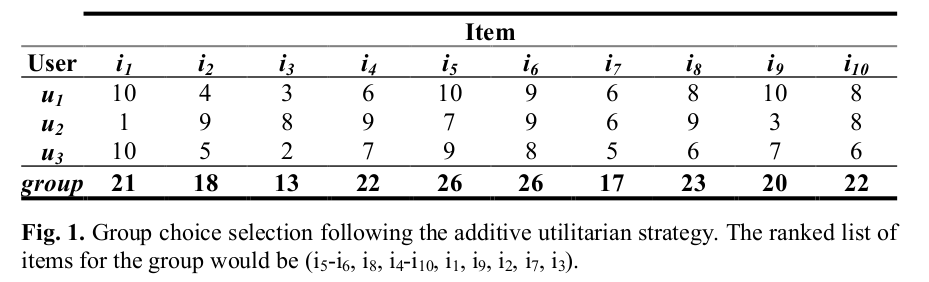
\includegraphics[scale=0.4]{images/additive.png}
\item[2)] \textbf{Average without misery strategy} : chaque item reçoit une note moyenne en fonction des notes données par les utilisateurs. Les items ayant reçus une note en dessous d'un certain seuil par au moins un utilisateur ne sont pas considérés pour la suite. Les autres items peuvent être classés.
\\
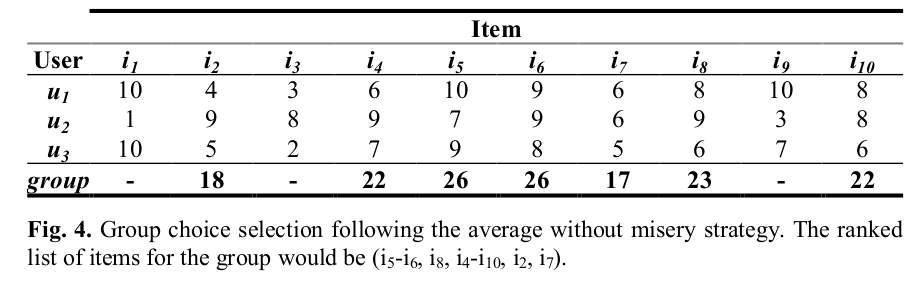
\includegraphics[scale=0.4]{images/average_without_misery.png}
\item[3)] \textbf{Least misery strategy} : chaque item reçoit comme note finale la moins bonne note donnée par les utilisateurs. Les items peuvent ensuite être classés. La satisfaction du groupe pour une musique est donc réduite à la satisfaction de l'utilisateur qui apprécie le moins cette musique.
\\
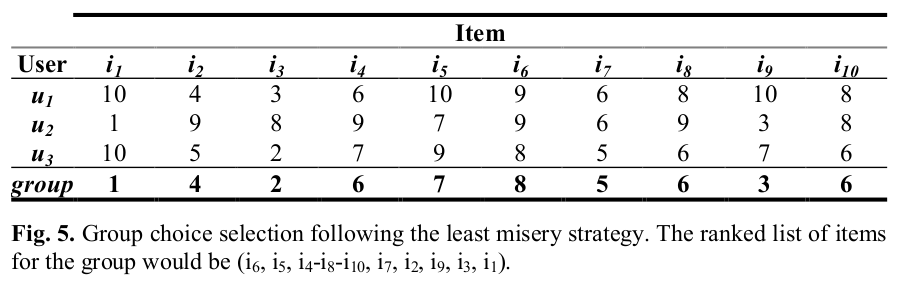
\includegraphics[scale=0.4]{images/least_misery.png}
\item[4)] \textbf{Fairness strategy} : les items les mieux notés d'un utilisateur pris au hasard sont sélectionnés. Parmi ces items, celui ayant reçu la meilleure note (par la \textit{least misery strategy}), reçoit la note maximale (qui correspond au nombre d'items). Ce processus est répété avec tous les autres items et la note reçue diminue de 1 à chaque fois. Les notes ainsi attribuées vont du nombre d'items à 1, ce qui effectue un classement.
\\
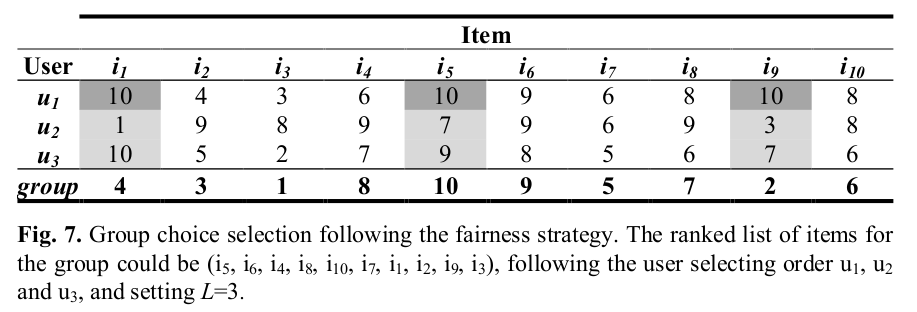
\includegraphics[scale=0.4]{images/fairness.png}
\item[5)] \textbf{Plurality voting strategy} : cette stratégie reprend le même principe que la \textit{fairness strategy}. La différence est que l'item sélectionné parmi ceux du premier utilisateur est celui qui a reçu le plus de votes par les autres utilisateurs.
\\
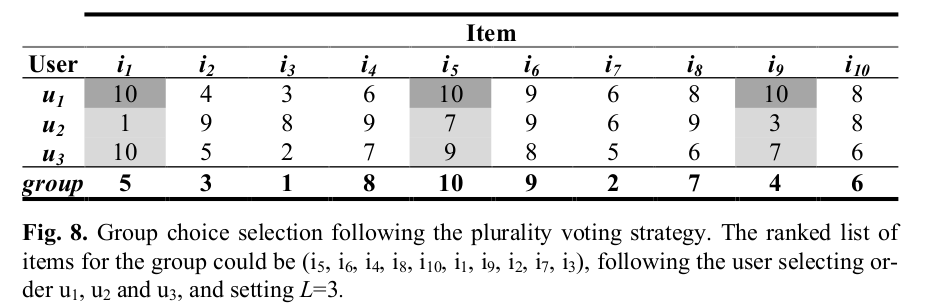
\includegraphics[scale=0.4]{images/plurality_voting.png}
\item[6)] \textbf{Borda count strategy} : les notes données par chaque utilisateur pour tous les items sont modifiées. Pour un utilisateur, l'item ayant reçu la moins bonne note reçoit une nouvelle note de 0. Les notes augmentent ensuite de 1 pour les items suivant. Les items ayant la même note initiale reçoivent tous la moyenne des nouvelles notes qui auraient du être attribuées. Par exemple, si deux items ont la même note et devraient recevoir les notes 2 et 3, ils reçoivent tous les deux la moyenne qui est de 2.5. Les nouvelles notes sont ensuite additionnées pour établir le classement.
\\
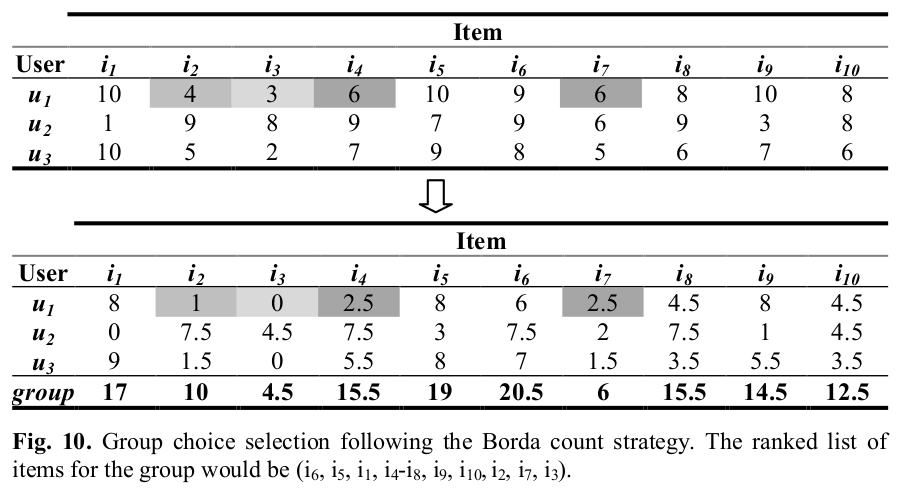
\includegraphics[scale=0.4]{images/borda_count.png}
\item[7)] \textbf{Copeland rule strategy} : cette stratégie repose sur la méthode de Copeland, c'est-à-dire que l'on réalise une comparaison par paire d'items. Au préalable, il est nécessaire de connaître le score attribué par rapport à chaque utilisateur pour chaque item. Il est possible de construire un tableau reposant ensuite sur le système suivant : 
\\
- si un item est considéré "meilleur" par rapport à ses scores attribués par \textbf{chaque utilisateur} qu'un autre item, alors cet item "bat" l'autre item, et on place un + dans la case correspondant à la comparaison entre ses deux items.
\\
- si un item est considéré "moins bon" par rapport à ses scores attribués par \textbf{chaque utilisateur} qu'un autre item, alors cet item est "battu" par l'autre item, et on place un - dans la case correspondant à la comparaison entre ses deux items.
\\
- si un item est considéré "aussi bon" par rapport à ses scores attribués par \textbf{chaque utilisateur} qu'un autre item, alors on place un 0 dans la case correspondant à la comparaison entre ses deux items.
\\
A partir du tableau construit par ce système, il est possible de calculer le score de chaque item par rapport au nombre de -, de + et de 0. Si l'on rencontre un +, alors le score de l'item en question augmente de 1, si l'on rencontre un -, alors le score diminue de 1, et si l'on rencontre un 0, le score reste inchangé. De là, nous obtenons le score pour chaque item, et les meilleurs items pour tous les utilisateurs selon la méthode de Copeland sont évidemment ceux qui ont le meilleur score.
\\
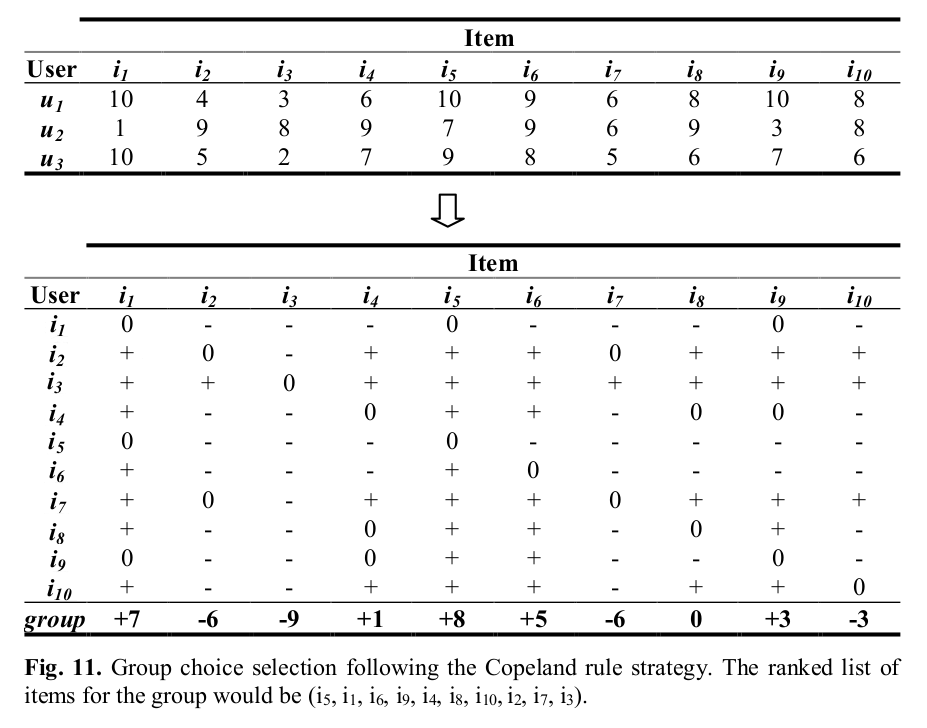
\includegraphics[scale=0.4]{images/copeland_.png}
\\

\end{itemize}

\section{Description des besoins}

\subsection{Liste des besoins fonctionnels}
Voici la liste non-exhaustive des différents besoins fonctionnels de l'application :
\subsubsection{Besoins essentiels}
\begin{itemize}
\item[1) -] Notre application doit assurer la \textbf{connexion de plusieurs utilisateurs} à leur compte Spotify. En d'autres termes, l'application doit être en mesure de gérer le fait que plusieurs personnes partagent leurs informations Spotify en même temps. Il y a un minimum de 1 utilisateur connecté et l'application doit pouvoir ajouter jusqu'à 10 utilisateurs. Une seule personne devra détenir l'application sur son téléphone. L'ensemble des utilisateurs voulant s'intégrer au groupe afin que leurs goûts musicaux soient pris en compte devront se connecter à leur compte Spotify sur le téléphone de l'utilisateur principal. De fait, l'application est dite "locale". Les goûts des utilisateurs seront pris en compte puisqu'à chaque ajout, l'algorithme de génération est relancé et propose une nouvelle playlist pouvant plaire à tous les utilisateurs. Pour le bon fonctionnement de l'application, il est impératif que l'utilisateur principal ait un accès à internet, que l'application Spotify soit installée sur son appareil, et que ce dernier soit sous le système d'exploitation Android.
\\
\\
Par rapport à l'ajout de plusieurs utilisateurs par authentification Spotify, il est possible de faire des tests sur l'ajout et par conséquent la mise à jour de playlist par relance automatique de l'algorithme. Le test se découpe de la façon suivante :
\begin{itemize}
\item[-] Récupérer la playlist courante.
\item[-] Création d'un objet utilisateur avec des fausses données (dans un modèle similaire à un cas d'utilisation normal de l'application quand première authentification/ajout d'utilisation).
\item[-] Appeler la fonction d'ajout sur cet utilisateur.
\item[-] Si l'utilisateur est ajouté dans l'application, alors techniquement il se trouve dans la liste courante des utilisateurs de l'application. Il faut alors procéder à un checking de la liste des utilisateurs et vérifier qu'il est bien à l'intérieur.
\item[-] Après l'ajout d'un utilisateur, selon la vision que nous avons faite de notre implémentation, l'algorithme se relance sur la liste courante des utilisateurs et une nouvelle playlist est générée en fonction des goûts des utilisateurs actuels, ce qui a pour conséquence d'écraser l'ancienne playlist.
\item[-] Pour finir, il faut vérifier que la playlist nouvellement générée est bien différente de l'ancienne playlist récupérée au début du test. Si c'est le cas, non seulement l'ajout utilisateur s'est bien effectué, mais en plus la mise à jour de la playlist a eu lieu par relance automatique de l'algorithme.
\\
\end{itemize}

\item[2) -] De pair avec le premier besoin, l'application doit permettre de \textbf{déconnecter un utilisateur à tout moment}. En effet, si une personne n'est plus présente sur le lieu de diffusion de la musique, il faut pouvoir retirer son compte afin que ses goûts n'influent plus sur les musiques diffusées. Il faut alors relancer l'algorithme de génération pour créer une nouvelle playlist.
\\

Pour le double test concernant la suppression d'un utilisateur/mise à jour d'algorithme, il s'inspire du même modèle que le test précédent.
\\
\\

\item[3) -] L'application doit pouvoir \textbf{accéder aux informations Spotify de chaque utilisateur} grâce à son API. Ces informations sont la base sur laquelle notre application va s'appuyer afin de proposer la solution souhaitée. Elles sont nécessaires à la mise en oeuvre des algorithmes de génération de playlist, mais aussi à leur bon fonctionnement. Ces informations sont diverses, telles que :
\begin{itemize}
\item[•] L'ensemble des playlists de l'utilisateur.
\item[•] L'ensemble des morceaux d'une playlist donnée.
\item[•] La chanson et son album correspondant.
\item[•] La chanson et son/ses artiste(s) correspondant(s).
\item[•] L'album et son/ses artiste(s) correspondant(s).
\item[•] Tous les titres musicaux que l'utilisateur a aimé.
\item[•] Les 50 derniers titres musicaux que l'utilisateur a écouté.

\end{itemize}
L'utilisateur doit donc pour cela autoriser l'application à accéder à ses informations Spotify.
\\
\\
Par rapport à ce besoin, on peut alors procéder à un test de récupération des données. Étant donné que théoriquement l'application fonctionne sur la base du token et de l'ID Spotify récupérés lors de l'authentification de chaque utilisateur, il est nécessaire de vérifier que le token et l'ID Spotify ont bien été récupérés (requêtes de type GET dont les réponses sont différentes de null). Après cette première vérification, si on est bien sûr d'avoir récupéré ces premières informations, il faut procéder à des tests de requêtes avec le Spotify ID et le token spécifiques à l'utilisateur. 
\\
Un test de requête type est de vérifier qu'on peut obtenir une playlist avec le Spotify ID de l'utilisateur, tout en vérifiant que cette playlist appartient bien à l'utilisateur (par l'intermédiaire de la clé unique user ID). Si c'est le cas, alors il est possible de récupérer toutes les autres informations grâce aux requêtes de type GET avec ce Spotify ID. S'il est possible de faire des requêtes avec ce Spotify ID, par déduction, il est possible de récupérer les informations Spotify de l'utilisateur.
\\
\\
\item[4) -] L'application doit être en mesure de pouvoir \textbf{proposer une ou plusieurs playlists adaptées aux goûts des utilisateurs}, grâce aux informations recueillies sur Spotify. 
\\
Pour ce faire, l'application va se baser sur différents algorithmes de génération de playlists, reflétant les stratégies trouvées au sein d'une des ressources à disposition du projet \cite{Algorithme}.
\\
Parmi ces stratégies, on préférera retenir celles dites de "least misery" qui consistent à privilégier des musiques qui sont plus ou moins appréciées par tout le monde plutôt que des musiques qui sont fortement appréciées par certaines personnes et très peu par d'autres.
\\
On pourra par exemple se baser sur un système de points qui permettra de noter les musiques, ou les styles de musiques en fonction des informations utilisateur récupérées. Plus un style de musique est écouté par différents utilisateurs, plus sa note sera élevée et inversement. Les musiques ayant les notes les plus élevées sont alors ajoutées à la playlist. On doit donc définir une taille par défaut pour les playlists afin de limiter le nombre de musiques n'ayant pas un score très élevé. Par défaut, ce paramètre sera initialisé à 50.
\\
\\
Il faudra tester ces algorithmes afin de vérifier que les musiques contenues dans la playlist générée sont bien compatibles avec les goûts des utilisateurs. Ces tests prendront en entrée un panel de musiques notées en fonction de la similarité de genre, d'artiste par rapport aux musiques écoutées habituellement par l'utilisateur et ce pour chaque utilisateur. Il prendra également en paramètre la stratégie à tester. Le but des algorithmes étant d'attribuer une nouvelle note à chaque musique et de garder les musiques ayant obtenues les meilleures notes, il faudra vérifier la compatibilité des notes finales avec les notes initiales. Pour ce faire on stockera le résultat attendu et on le comparera au résultat retourné par l'algorithme.
\\
\\

\item[5) -] L'application doit \textbf{assurer les fonctions de lecture de base} : lecture et pause des playlists générées par nos algorithmes, ainsi que la possibilité de "skipper" des titres musicaux. L'utilisateur devra avoir accès rapidement à une page sur l'application assurant ces fonctions. Pour que les musiques puissent être jouées, l'application Spotify doit être installée sur le mobile du détenteur de l'application.
\\
\\
\item[6) -] Elle offre la possibilité de \textbf{sauvegarder les logs d'écoute} liés à l'utilisation de l'application. Ces logs permettront de générer des statistiques réclamées par le client. 
\\
Il sera alors nécessaire de créer un panel permettant au client d'accéder à l'ensemble des statistiques de l'application. Pour pouvoir y accéder, le client pourra utiliser un nom d'utilisateur et un mot de passe dans le modèle admin-like.
\\
\\
Pour sauvegarder les logs d'écoute, il y a plusieurs possibilités qui permettent de sauvegarder les données en local, et nous avons gardé parmi ces moyens deux types de stockage de données, à choisir parmi :
\begin{itemize}
\item[-] Une base de données SQLite.
    SQLite est un moteur de base de données simple qui offre les fonctionnalités de base de données sans avoir besoin d'installer un logiciel complexe et l'installation d'un serveur de base de données. C'est un système de gestion de base de données relationnelle comme PostgreSQL ou MYSQL dont il diffère par le regroupement en un seul fichier de toutes les tables. SQLite est bien adapté pour les petits projets.
\item[-] Stockage au format JSON.
    La syntaxe de Json est dite orientée objet et permet aux langages de transformer facilement des données de l'objet JSON vers le langage courant. Comme la syntaxe est petite et légère, le temps d'exécution pour la réponse est très rapide. Un inconvénient de JSON est que sa syntaxe ne permet de gérer les cas d'erreurs.
\\
\\
\end{itemize}

Une méthode de test pour les logs d'écoute pourrait être de vérifier que la base de données est bien fonctionnelle et qu'elle est bien modifiée en fonction des interactions avec cette dernière (insertion/suppression/mise à jour des données). Pour cela, on testera chaque requête de la base de données, et on vérifiera que les données issues des logs d'écoute sont bien stockées, notamment par visualisation de la base de données ou par requête de GET sur des logs que l'on a inséré/supprimé.

\end{itemize}

\subsubsection{Besoins conditionnels}
\begin{itemize}
\item[1) -]Afin d'améliorer la génération des playlists, l'application pourra proposer des boutons de "like" et "dislike" permettant à chaque utilisateur d'indiquer s'il a ou non apprécié la musique diffusée. En fonction des likes et dislikes, il est possible de mieux évaluer nos algorithmes, et in fine générer des statistiques par rapport aux évaluations laissées par les utilisateurs.

\item[2) -]Quand une playlist est écoutée, la musique doit continuer d'être jouée même si l'écran n'est pas allumé. L'application continue de tourner quand le téléphone est verrouillé, mais pas éteint. 

\item[3) -]Afficher une page depuis la page principale qui permettra de modifier quelques paramètres de l'application tels que : \\
- La taille de la playlist, soit le nombre de titres musicaux qu'elle contient. \\
- La possibilité de choisir le mode de génération de la playlist entre automatique et manuel. Le mode automatique consiste à laisser le système de l'application choisir l'algorithme qui pourrait générer une playlist correspondant au mieux aux goûts de tous les utilisateurs. Le mode manuel permet de laisser à l'utilisateur le choix de l'algorithme de génération.

\end{itemize}
\subsubsection{Besoins optionnels}
\begin{itemize}
\item[1) -]La taille de la playlist est fixée à 50 par défaut. Elle pourra être modifiée dans les paramètres de l'application afin de varier entre 10 et 100 titres. Pour une moyenne de 4 minutes par musique, cela correspond à une durée de playlist entre 40 minutes et quasiment 7 heures.

\item[2) -]L'application pourra permettre d'afficher à quels utilisateurs la musique est la plus susceptible de plaire. Les utilisateurs peuvent ainsi avoir une explication du choix de la musique pour le groupe.

\item[3) -]L'application peut avoir une interface améliorée. Par exemple, pendant qu'une musique est écoutée, la pochette de l'album correspondant s'affiche.

\item[4) -]Il est possible de choisir Deezer ou Spotify pour se connecter.

\item[5) -]Il est possible d'afficher la playlist courante à partir de la page principale afin de voir quelles sont les musiques contenues dans cette playlist, ce qui permet de connaître les prochaines musiques qui seront diffusées ou celles qui sont déjà passées.

\end{itemize}

\subsection{Liste des besoins non-fonctionnels}

Voici la liste non-exhaustive des différents besoins non-fonctionnels de l'application.

\subsubsection{Fiabilité}

Notre application doit être \textbf{fiable}. Il est nécessaire d'assurer la fiabilité de l'application, afin d'offrir à l'utilisateur une expérience optimale. Pour cela, il faut procéder à des tests de fiabilité. Ceux-ci reviendront à cartographier les parcours utilisateurs clés, c'est-à-dire identifier toutes les étapes du parcours utilisateur et vérifier qu'il ne rencontrera aucun obstacle dans l'utilisation de l'application. 

\subsubsection{Sécurité}
Afin de sécuriser l'application et de minimiser son exposition aux menaces, pour que les données personnelles des utilisateurs soient protégées, l'application doit :
\begin{itemize}
    \item[•] proposer un système d'authentification par identifiant et mot de passe pour \textbf{l'admin}. 

    \item[•] contrôler l'accès des utilisateurs : un utilisateur souhaite accéder à une fonctionnalité, il faut contrôler s'il a le droit d'y accéder. En effet les logs d'écoute devant être récupérés, seule les personnes habilitées à récupérer ses informations devront avoir un rôle privilégié leur permettant d'accéder à ses informations particulières.
    
    \item[•] assurer la confidentialité des données lors d'échange de données sensibles comme les mots de passe. Il faut assurer que si des données sont acquises illégalement, elles soient inutilisables. La confidentialité peut être mise en oeuvre par un mécanisme de chiffrement permettant de protéger l'échange et le stockage des données.

\end{itemize}

\subsubsection{Facilité d'accès}

Notre application doit être \textbf{facile d'accès}. En d'autres termes, l'application doit être en mesure de proposer le moins d'interactions utilisateurs possibles pour qu'il arrive à ses fins. Comme dans la plupart des développements de projet qui veulent s'ancrer dans la facilité d'accès, on se fixe un maximum de trois interactions entre l'entrée de l'utilisateur sur l'application jusqu'à son objectif final.

\subsubsection{Performance}

Il est nécessaire que l'application soit \textbf{performante}. Dans la mesure où l'on veut que l'utilisateur puisse arriver à son objectif en un minimum de temps, nous devons nous assurer que le temps de réponse après une interaction utilisateur soit le plus faible possible. Le temps maximal de latence pour le chargement d'une page ne devra pas excéder 2 secondes. 

Par ailleurs, puisque nous utilisons des algorithmes de génération de playlists, nous devrons également limiter l'impact du temps de calcul de ces algorithmes dans l'application afin de ne pas altérer l'expérience utilisateur.

Des tests par rapport aux temps de réponse après chaque interaction devront être effectués tout au long de l'implémentation de l'application, afin de veiller à ce que celle-ci reste performante.

\subsubsection{Portabilité}

 Notre application doit être \textbf{portable sur mobile}. La finalité est que celle-ci soit utilisable sur un téléphone Android, cela en fait un des besoins non-fonctionnels majeurs de notre projet. \cite{API}
 
 \subsection{Illustrations par rapport aux différents besoins énoncés}
 
 \subsubsection{Diagramme des fonctionnalités de l'application}
 
 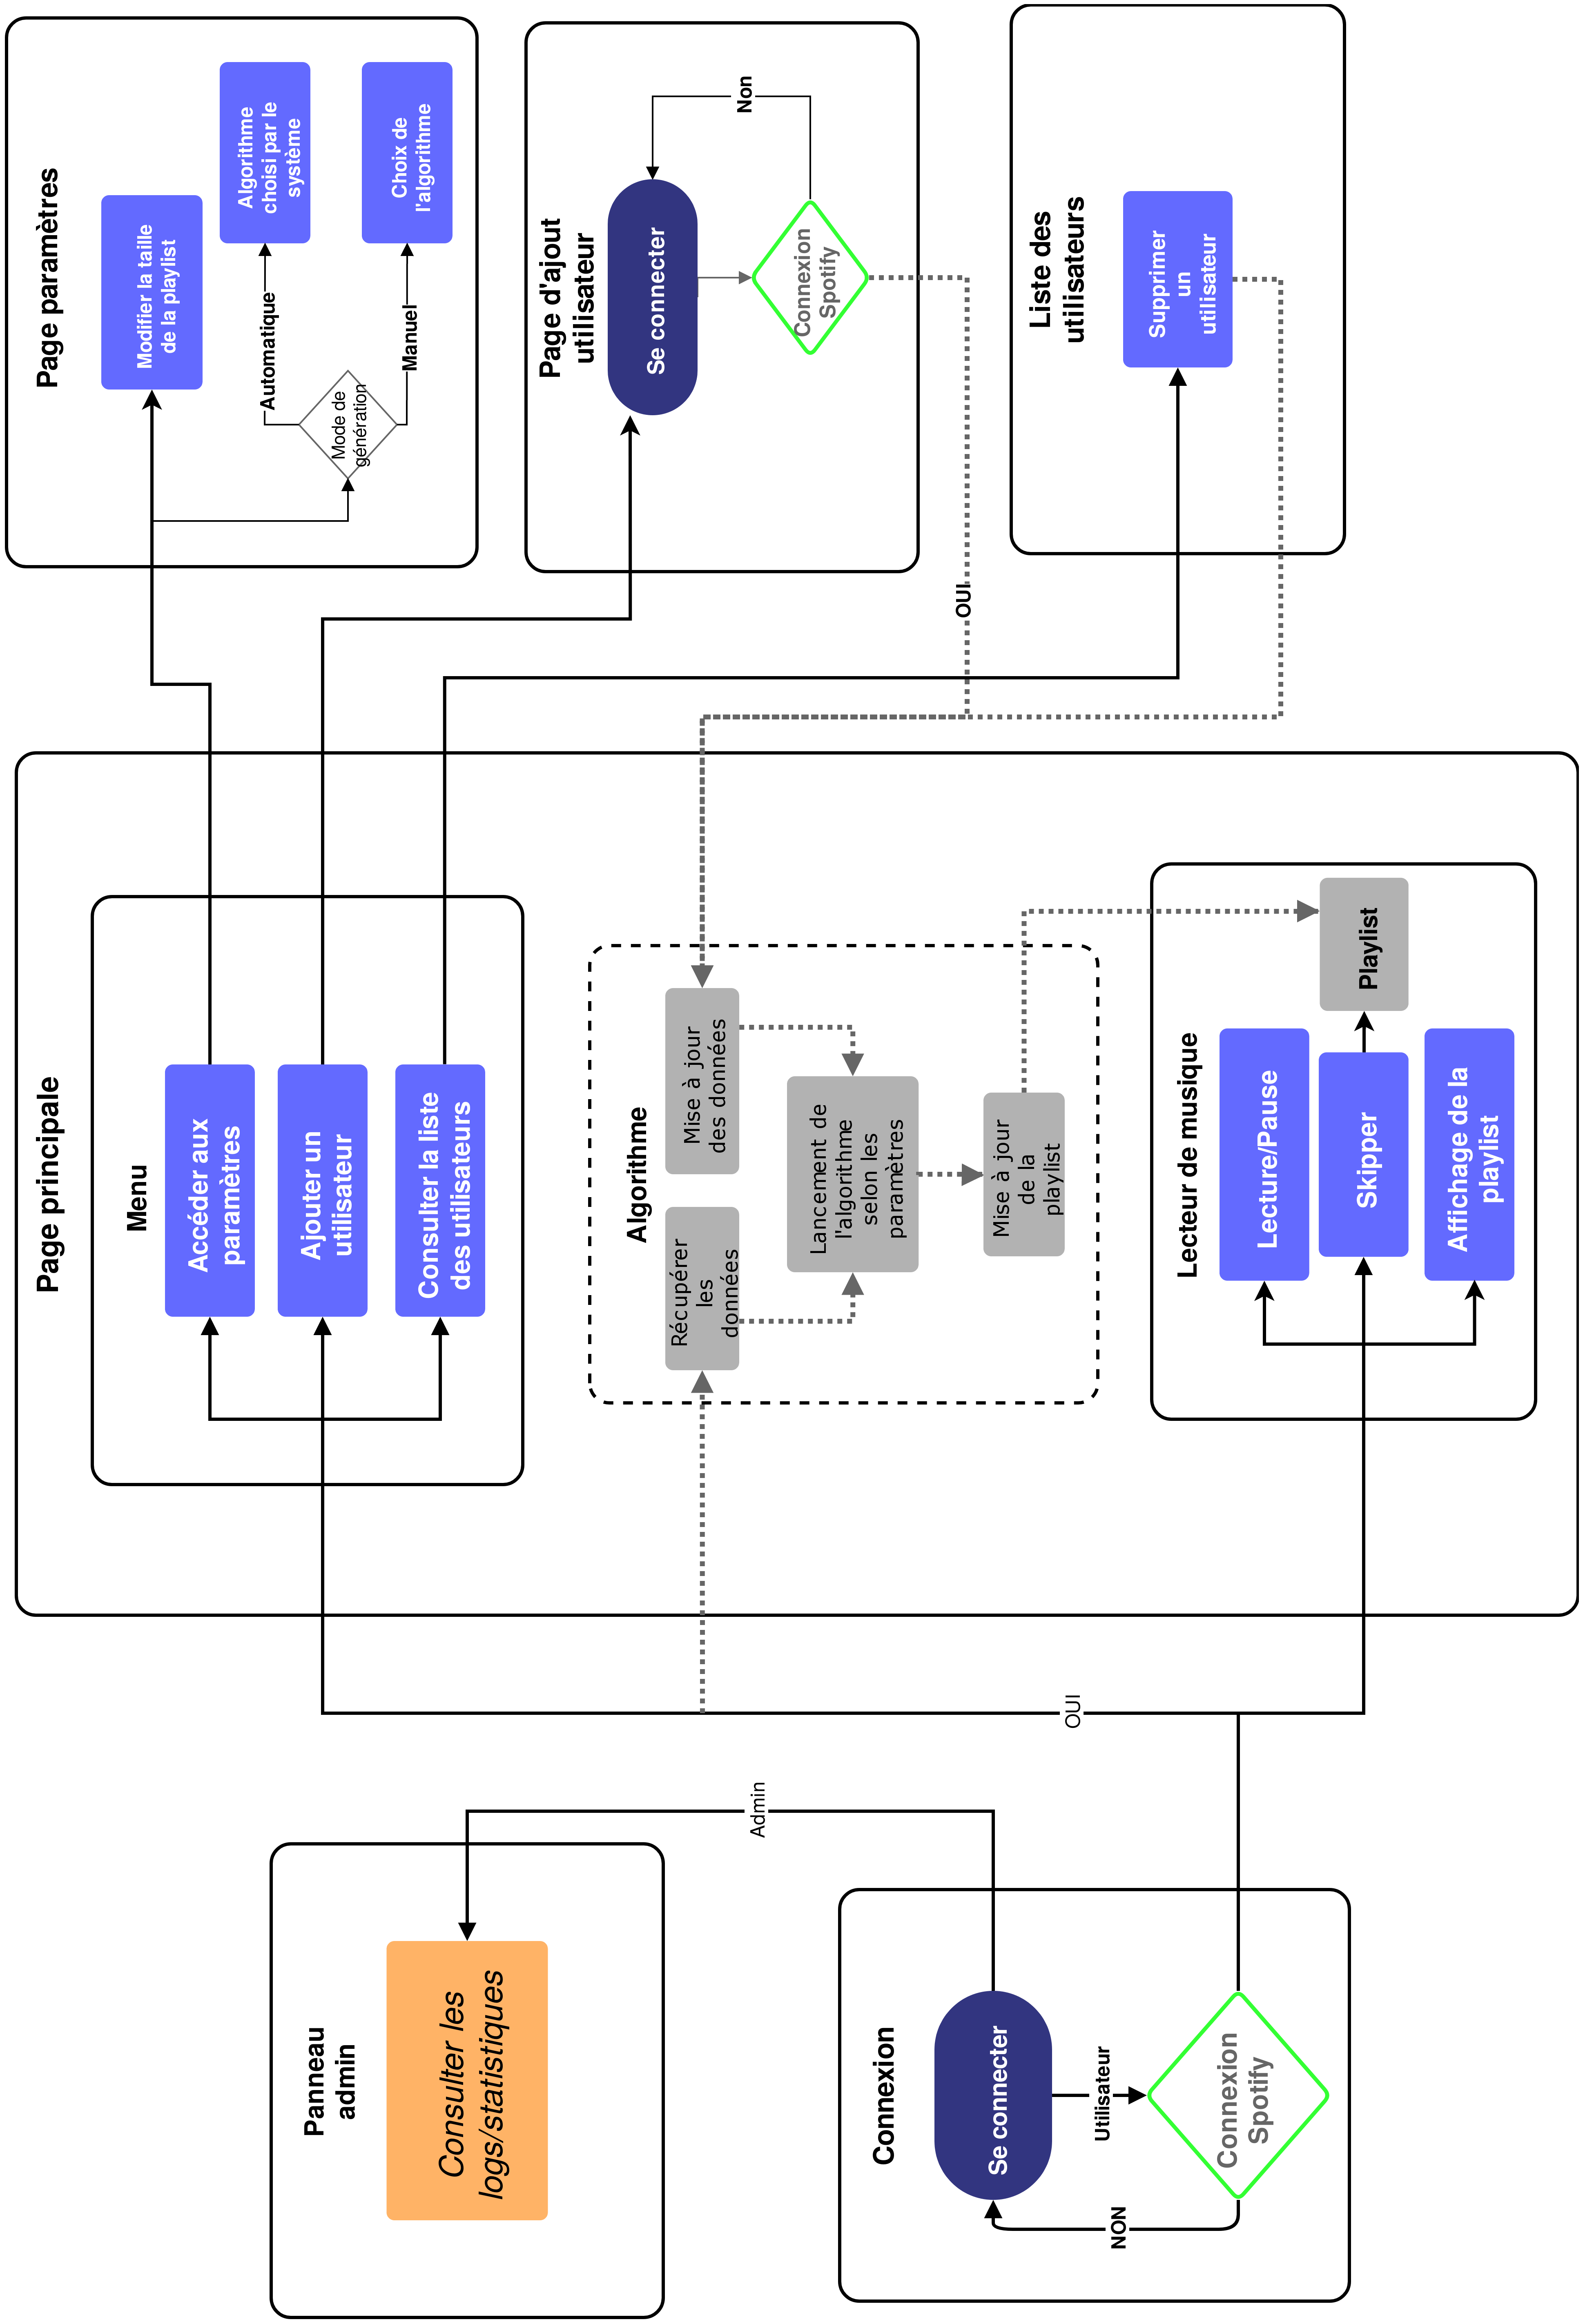
\includegraphics[scale=0.11]{images/schema_fonc.png}
 
 \subsubsection{Scénario d'utilisation}
 
  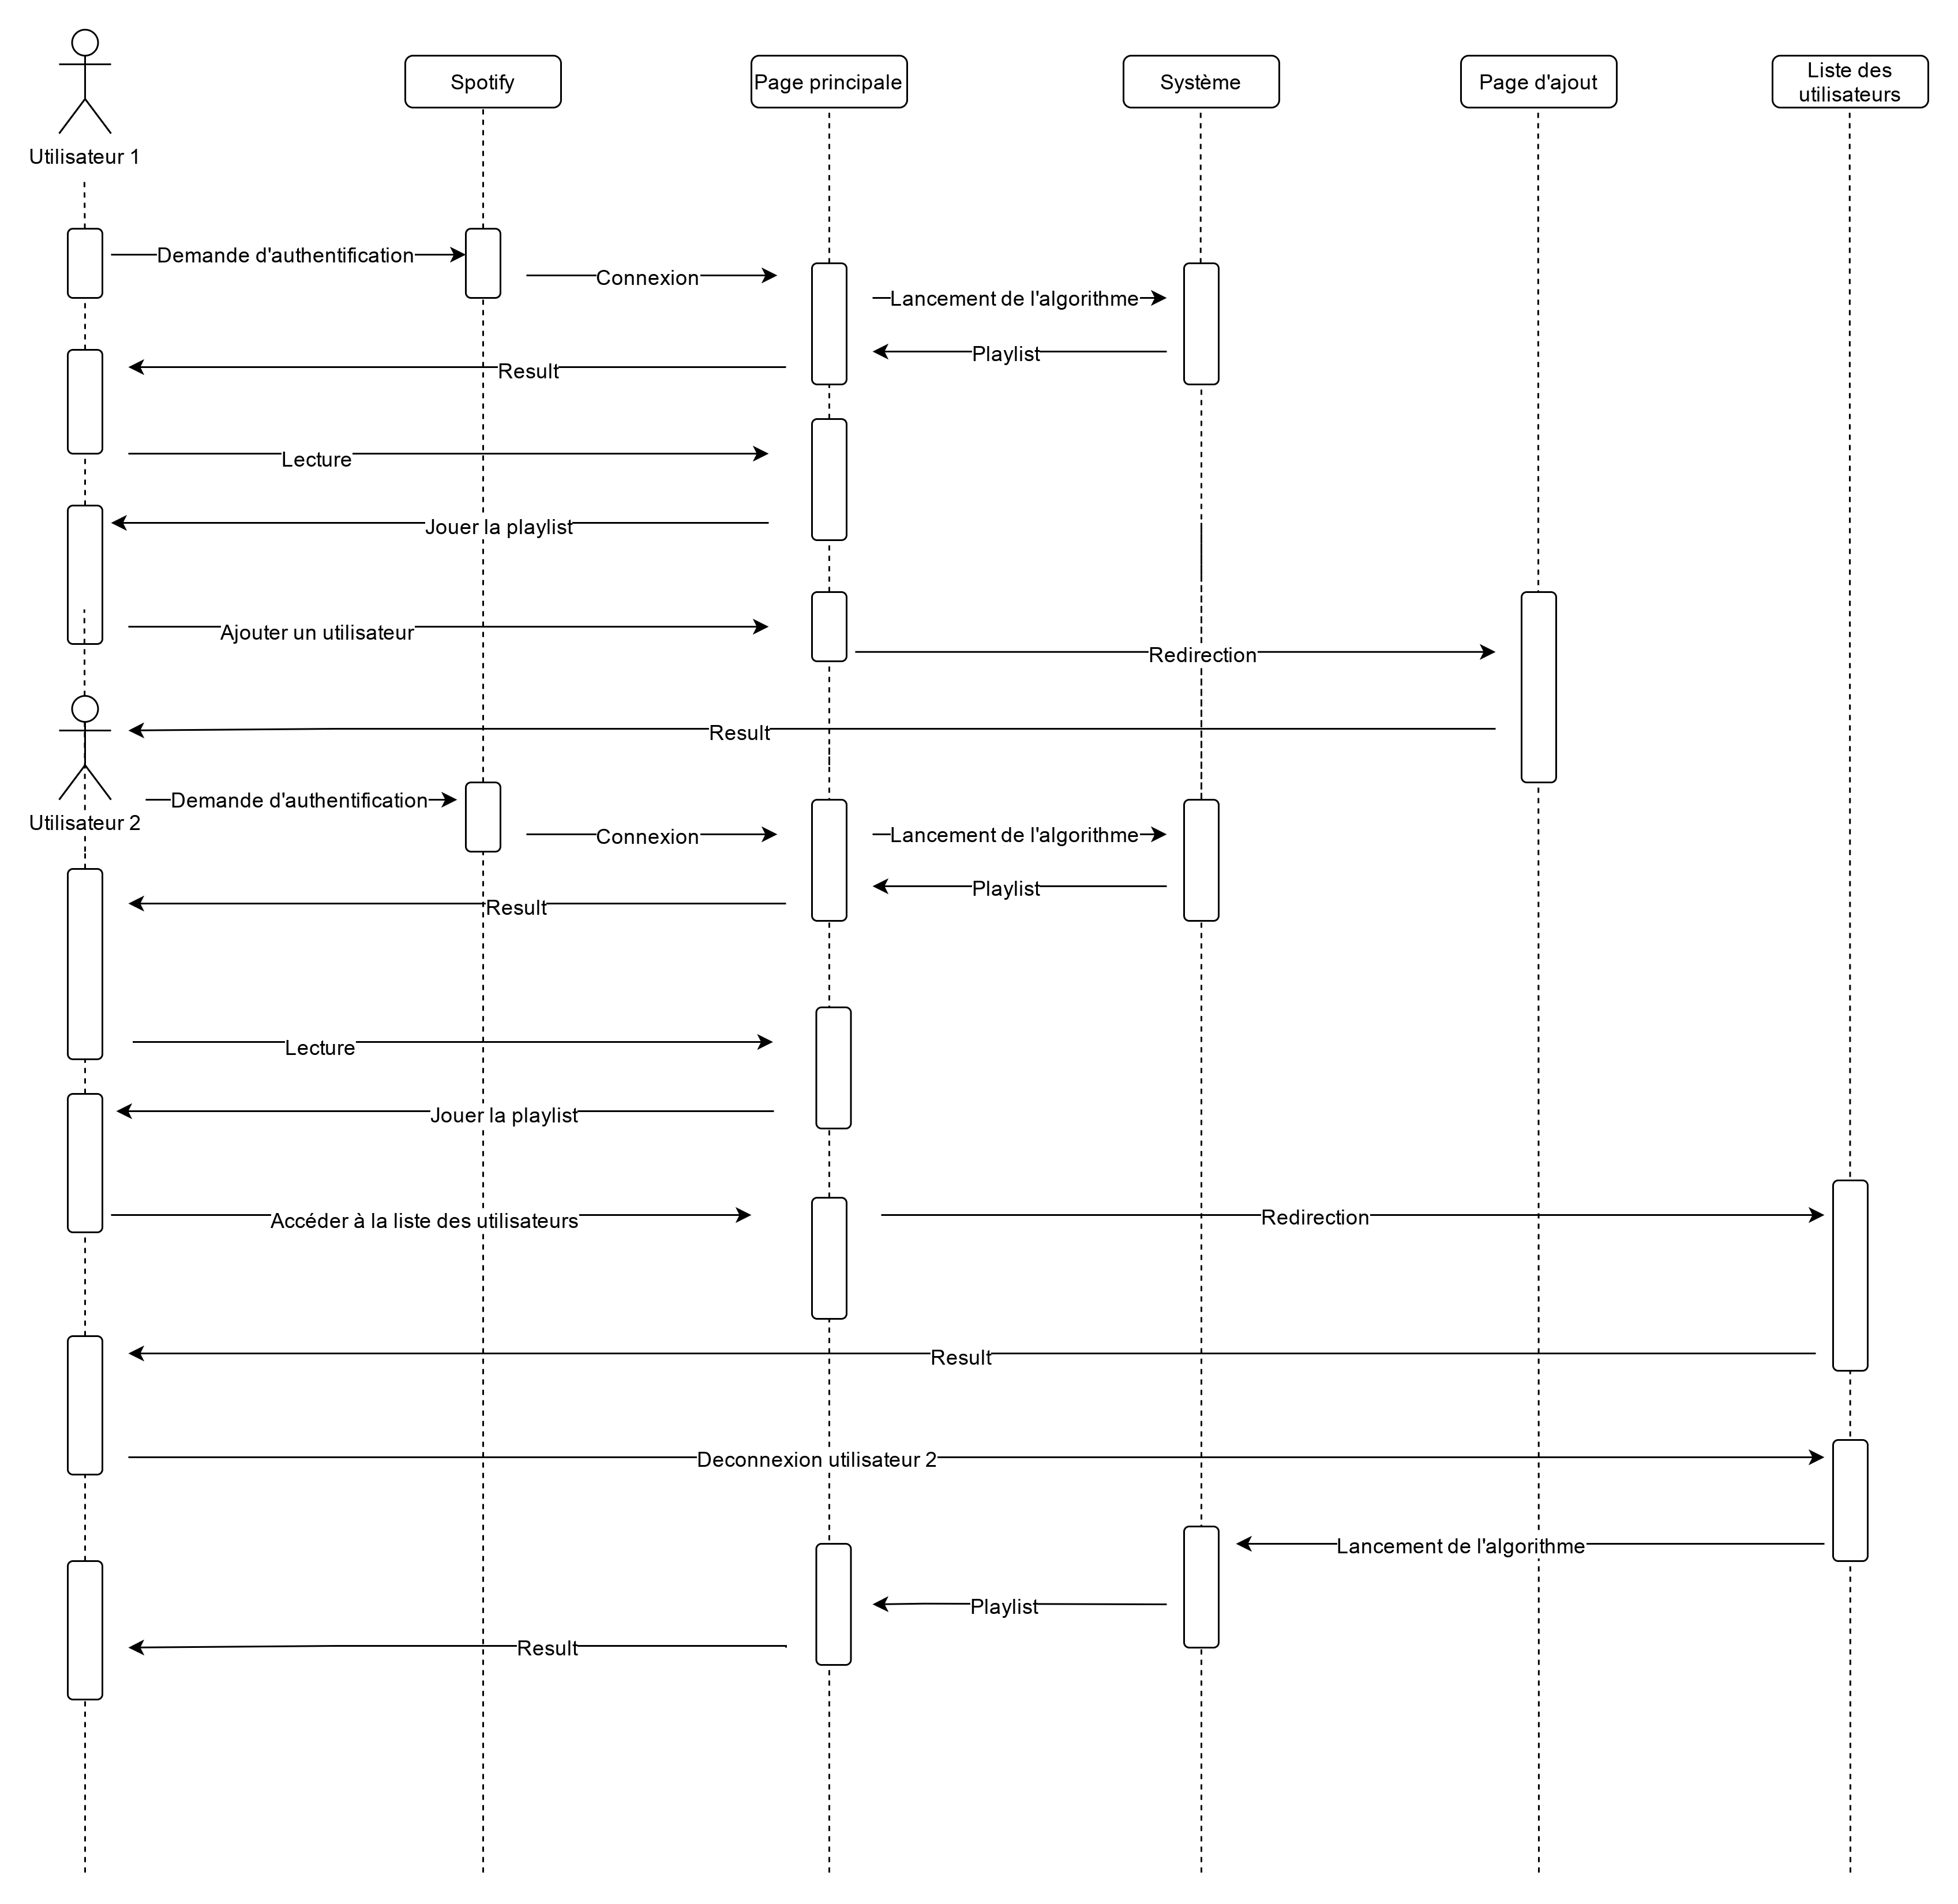
\includegraphics[scale=0.15]{images/scenar_user.png}
  
  \subsubsection{Diagramme de cas d'utilisation UML}
  
  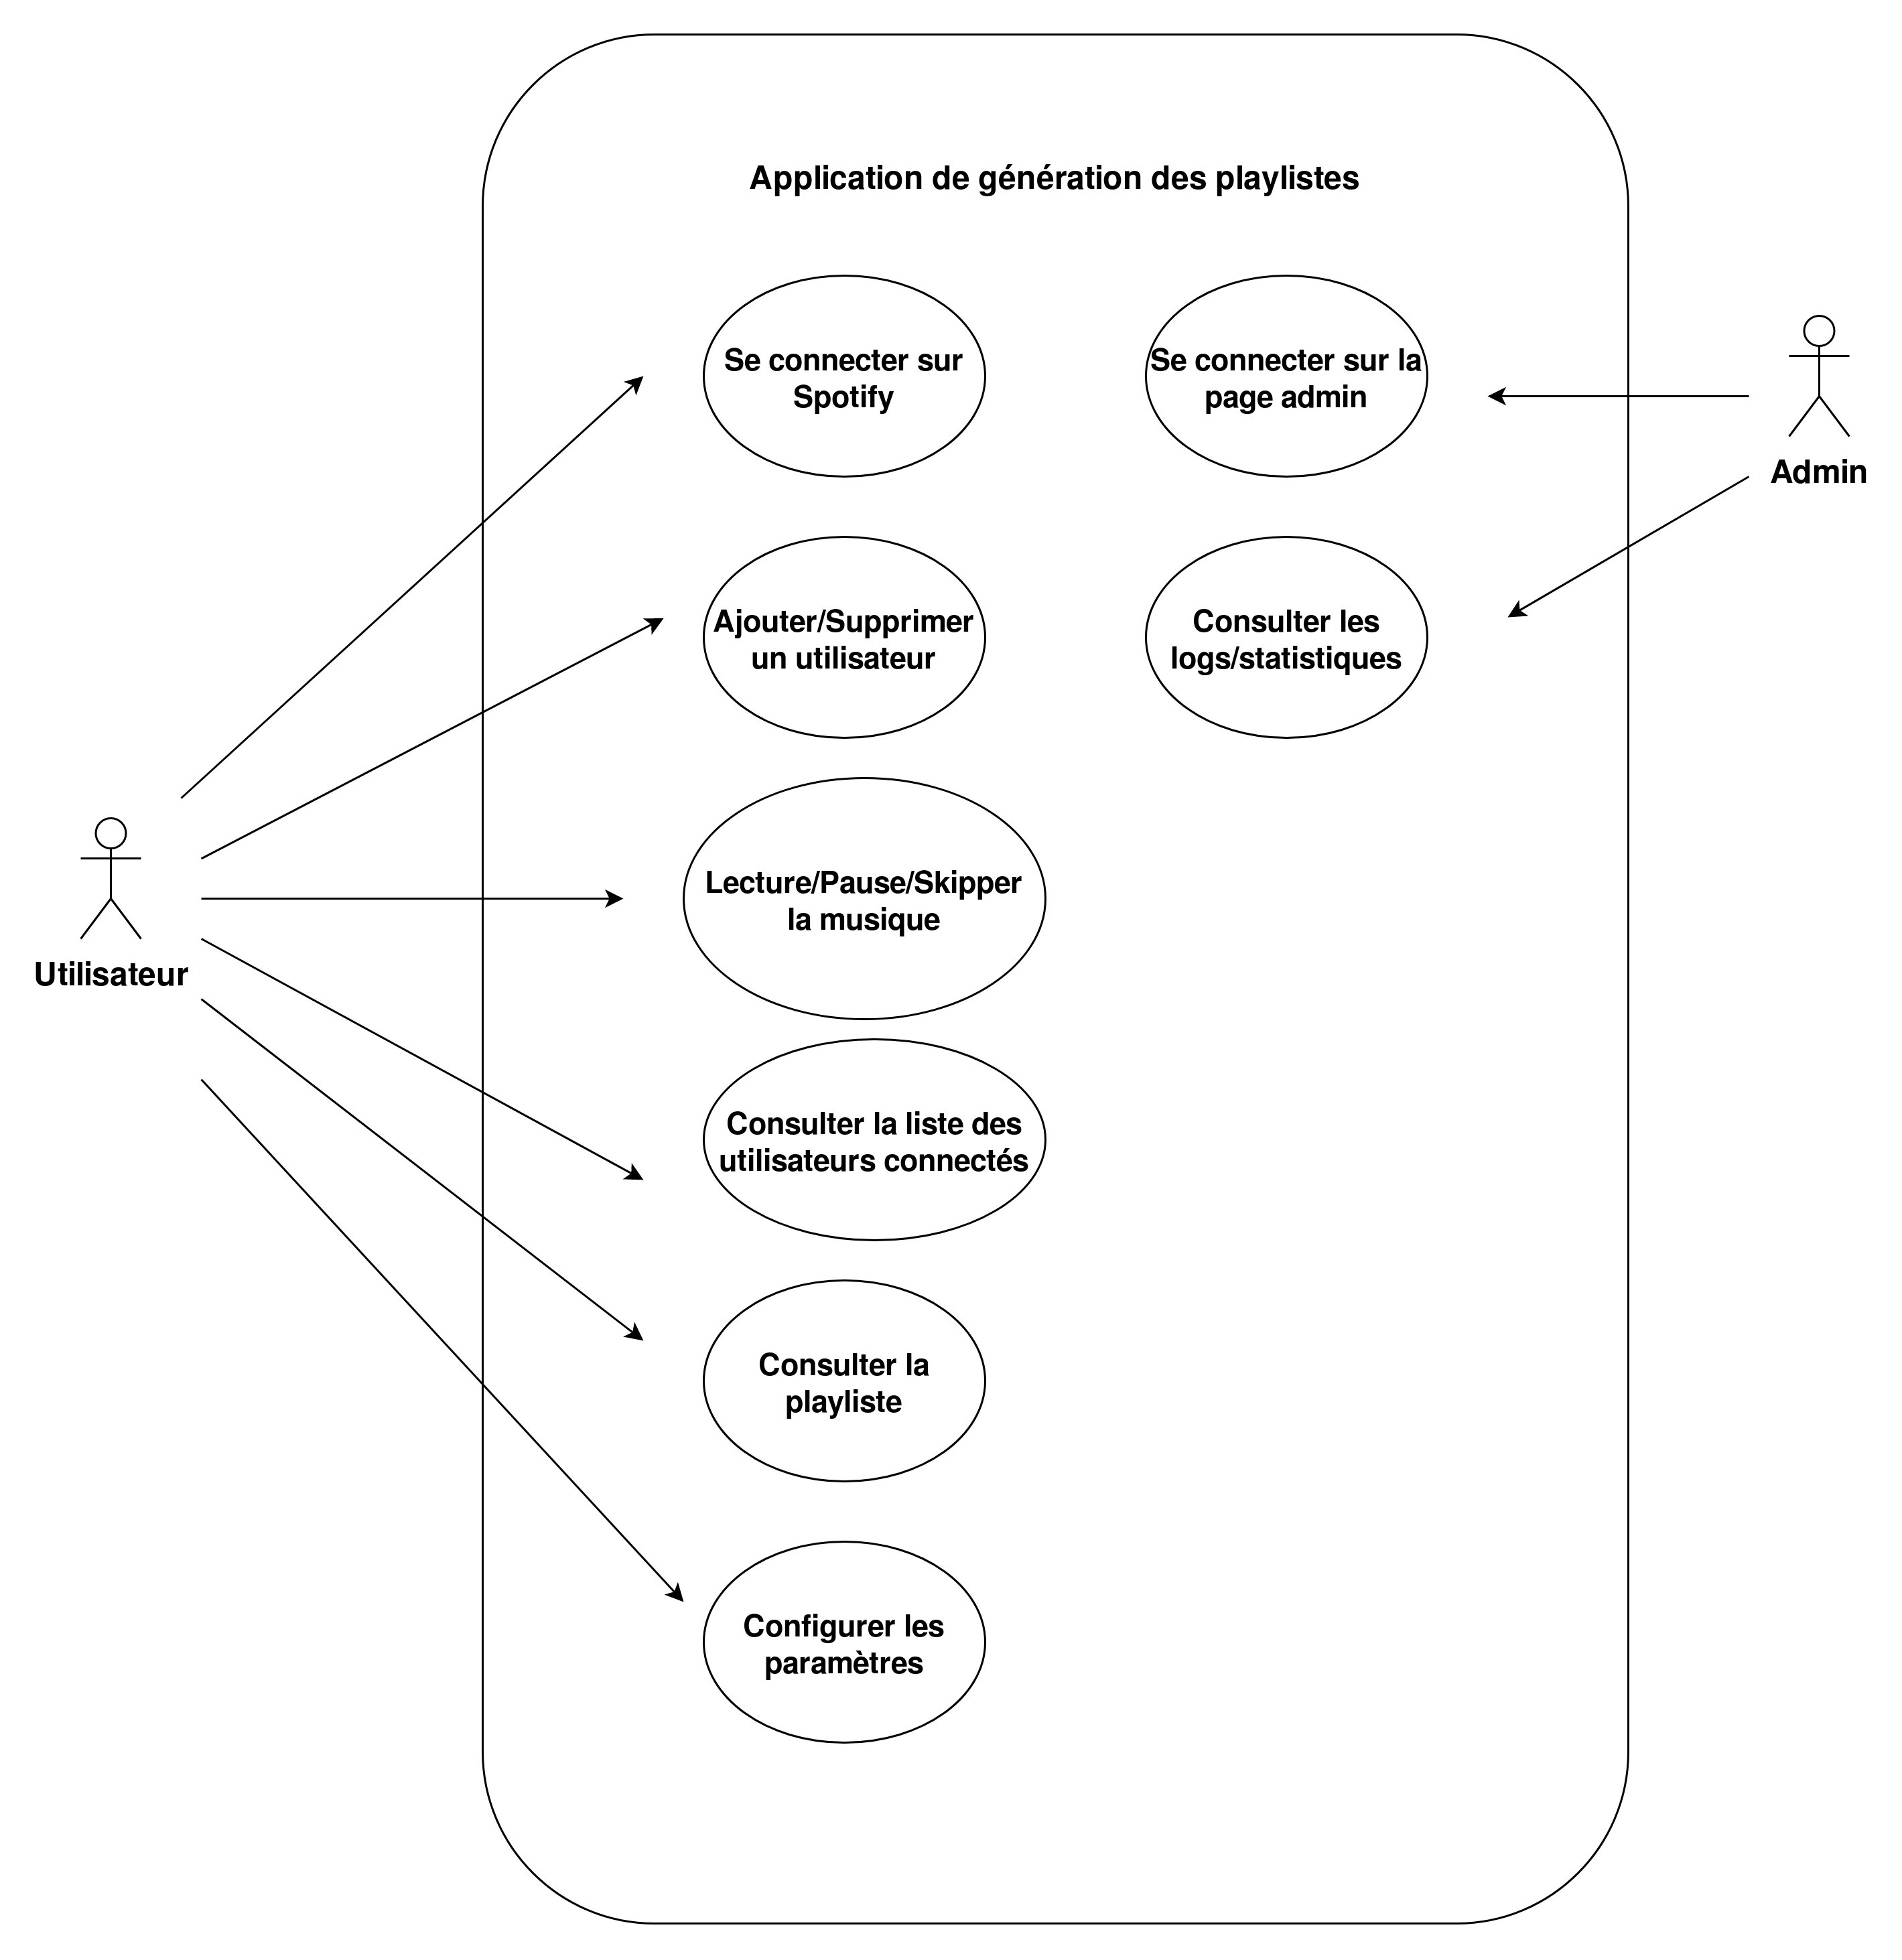
\includegraphics[scale=0.17]{images/cas_dutilisation.png}
  
 \subsubsection{Diagramme de faisabilité par rapport à la récupération des données}
   
   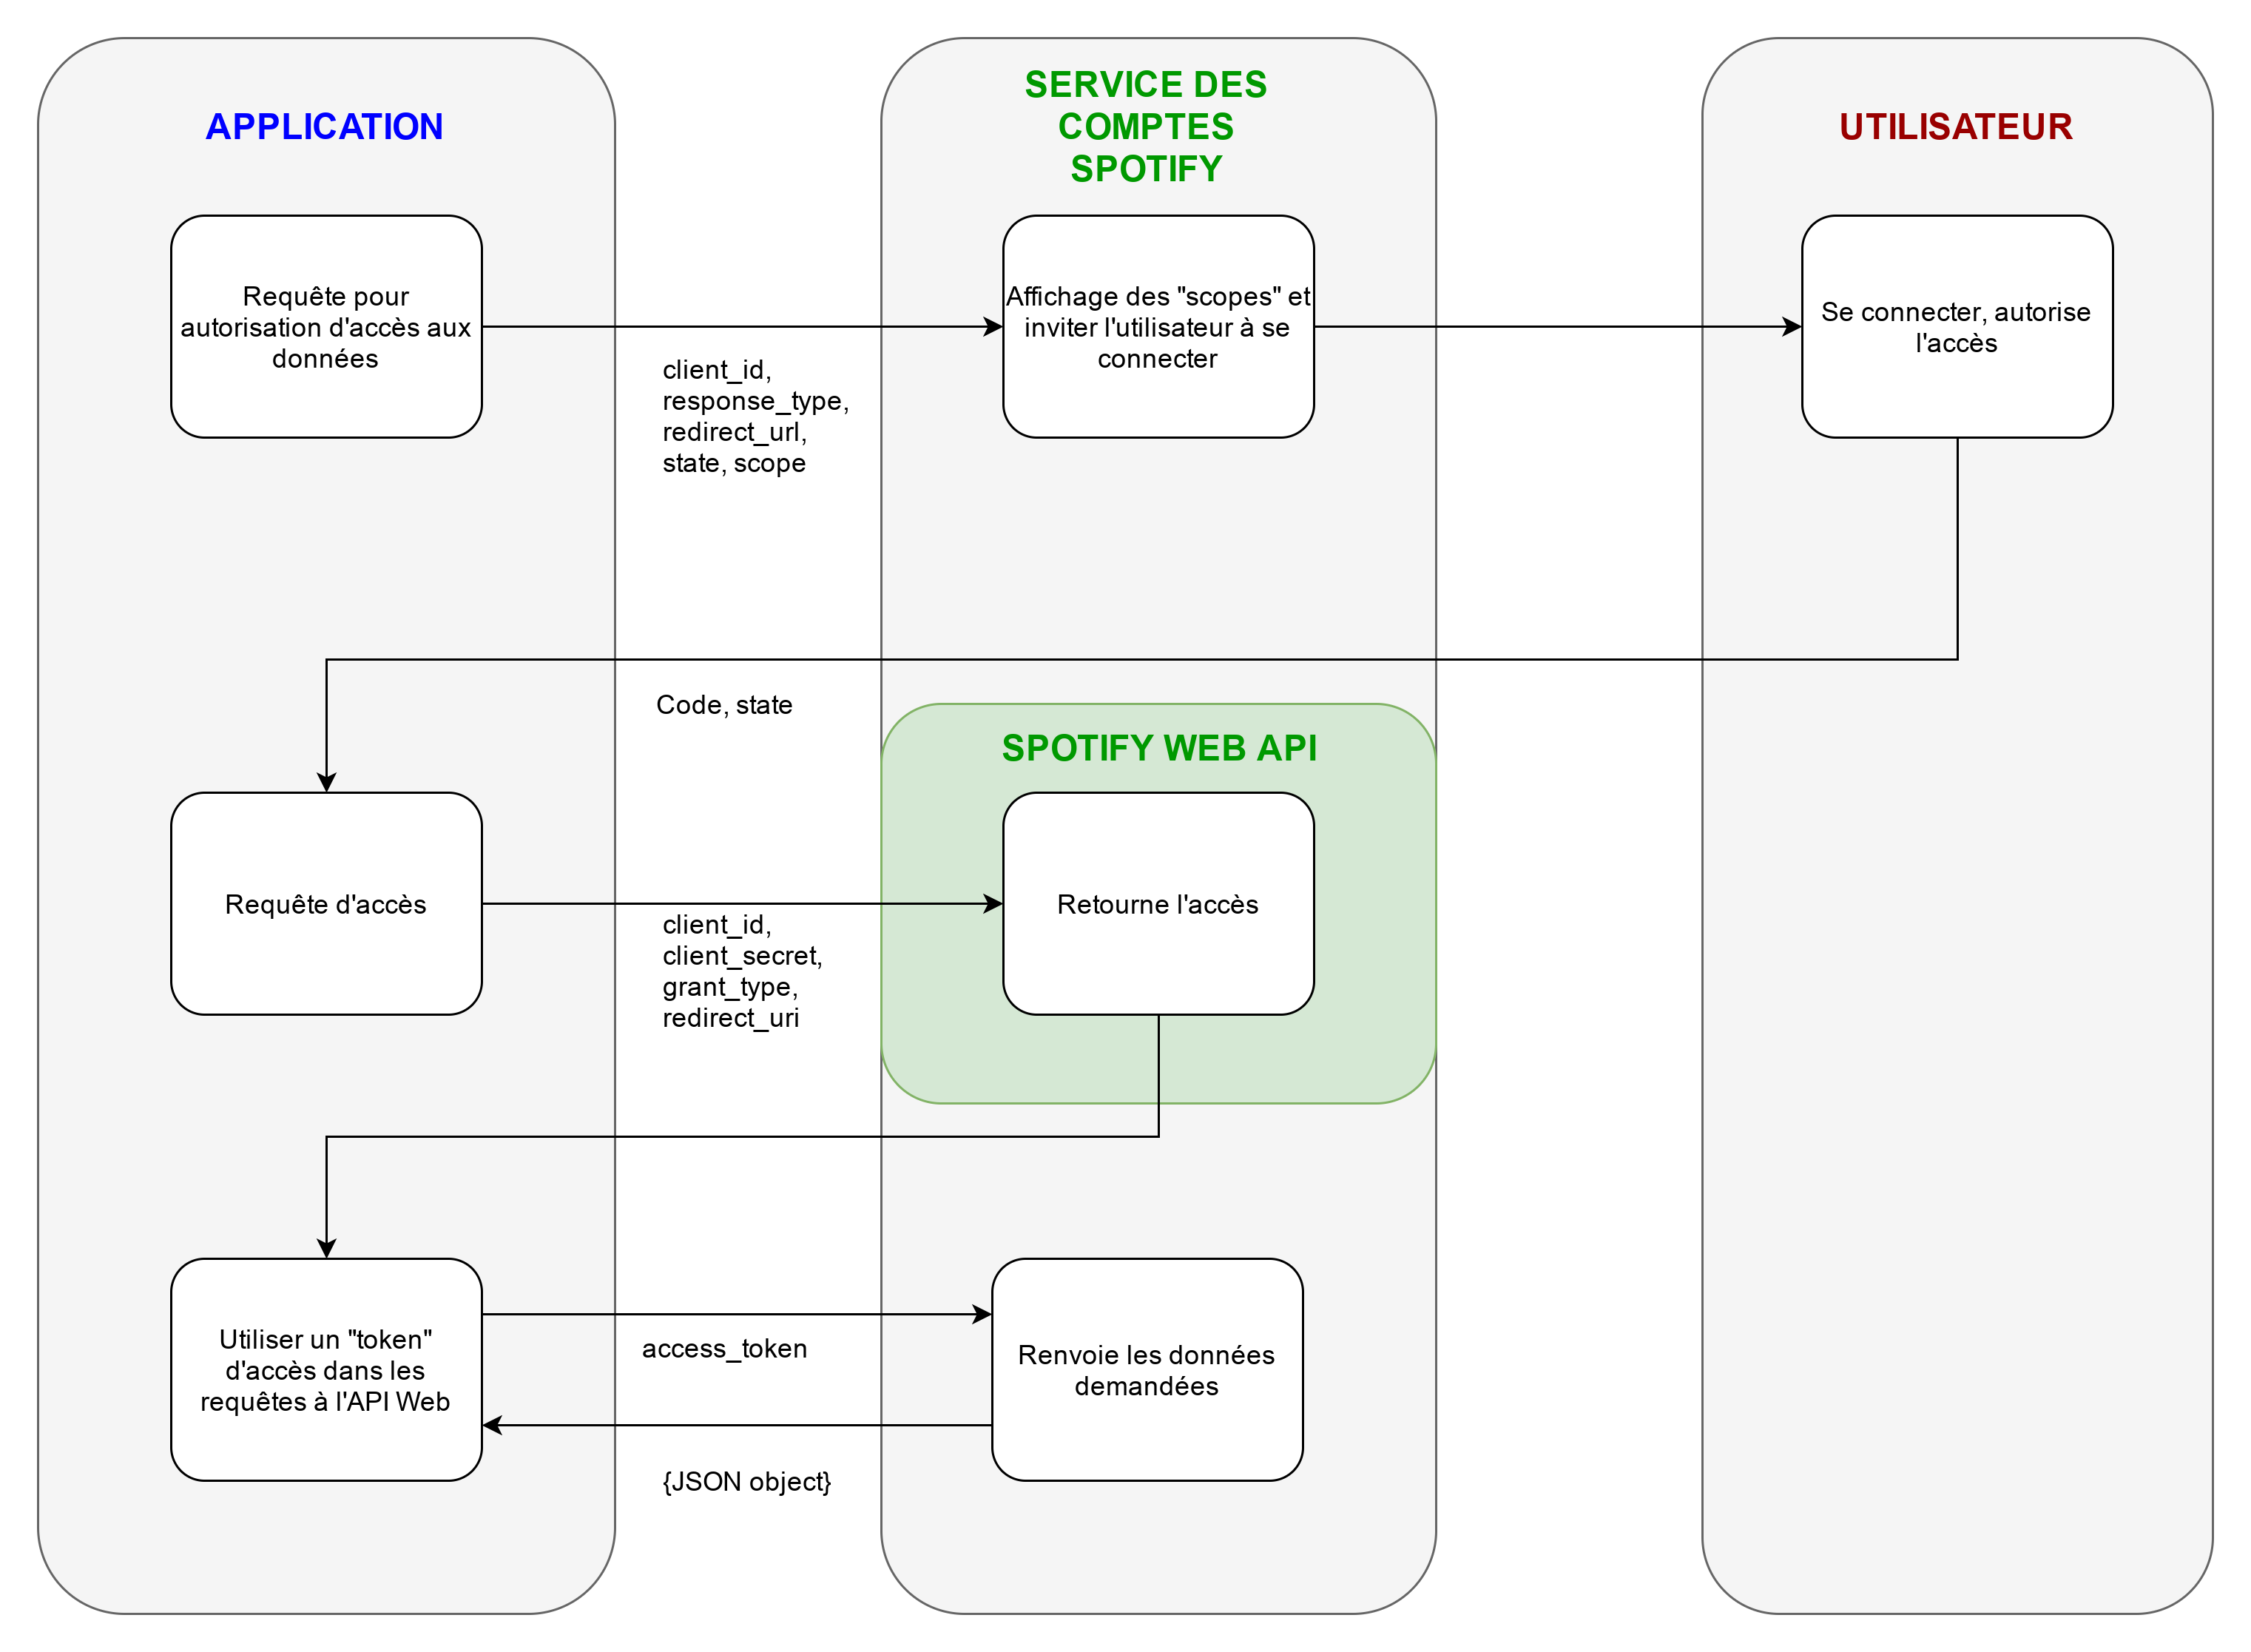
\includegraphics[scale=0.17]{images/schema_faisa_1.png}
   
   \newpage
   
 \subsubsection{Screens sur la possibilité de récupérer les données Spotify}
 
    Afin de démontrer la faisabilité du projet, nous avons d'ores et déjà implémenté, en plus du projet principal, une partie de code permettant de récupérer les données Spotify. Nous les affichons ensuite pour démontrer notre propos. Ci-dessous, le premier screen redirigeant vers une authentification sur l'application Spotify.
    \\
    \\
 
    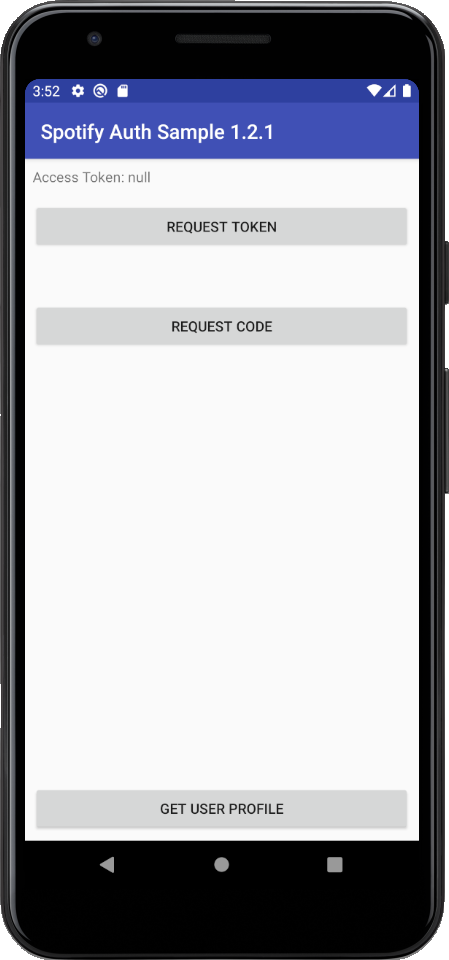
\includegraphics[scale=0.5]{images/recupinfos.png}
    
    \newpage
    
    Après la redirection sur la page d'authentification Spotify, il est nécessaire que l'utilisateur entre son mail et son mot de passe. Ces données ne relèvent pas de notre application, puisque c'est bien grâce à l'API de Spotify que l'authentification a lieu. En terme de sécurité, c'est donc Spotify qui s'occupe de bien vérifier l'authentification de l'utilisateur, et de s'occuper du chiffrement des données envoyées. \cite{Auth}
    \\
    \\
    
    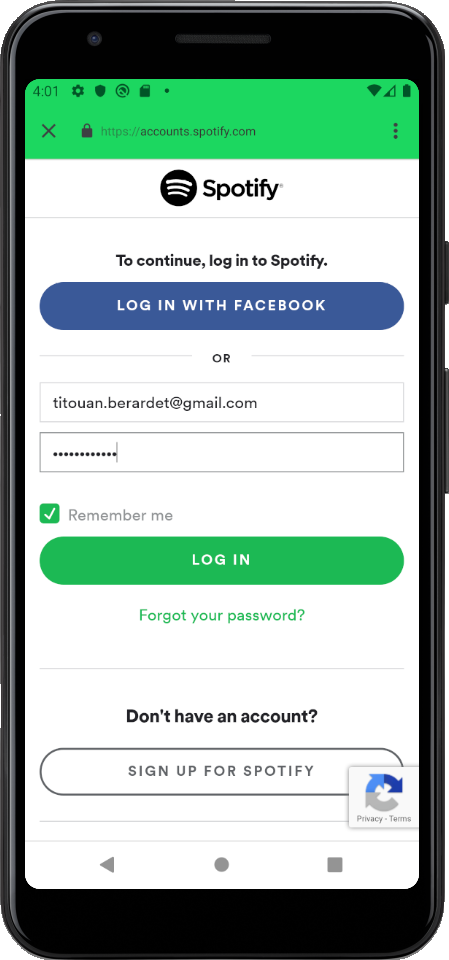
\includegraphics[scale=0.5]{images/authentification_exemple.png}
    
    \newpage
    
    Après l'authentification, Spotify demande à l'utilisateur s'il autorise l'application à accéder à ses données, en plus d'accéder à ses dernières activités sur Spotify.
    \\
    \\
    
    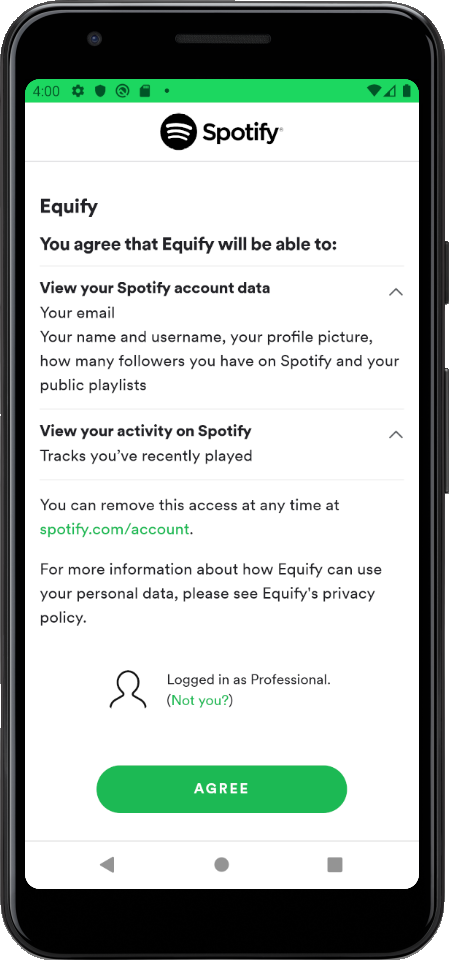
\includegraphics[scale=0.5]{images/accord_spotify.png}
    
    \newpage
    
    A partir de là, nous faisons des requêtes de type GET par l'intermédiaire de l'API Spotify, afin de récupérer un fichier JSON contenant les premières informations permettant de faire tourner le reste de l'application, soit l'ID Spotify et le token de l'utilisateur. Nous les affichons sur l'image ci-dessous, afin d'attester de la véracité de nos propos.
    \\
    \\
    
    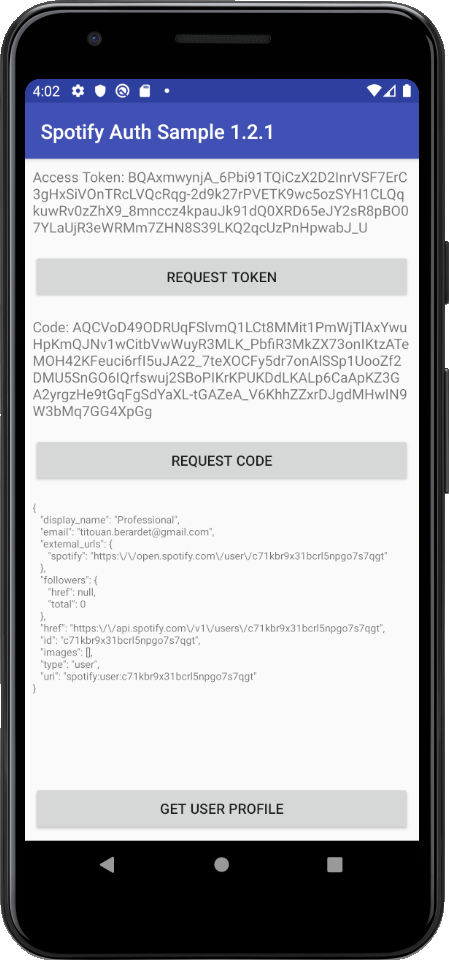
\includegraphics[scale=0.5]{images/informations.png}
    


\section{Diagramme de Gantt}


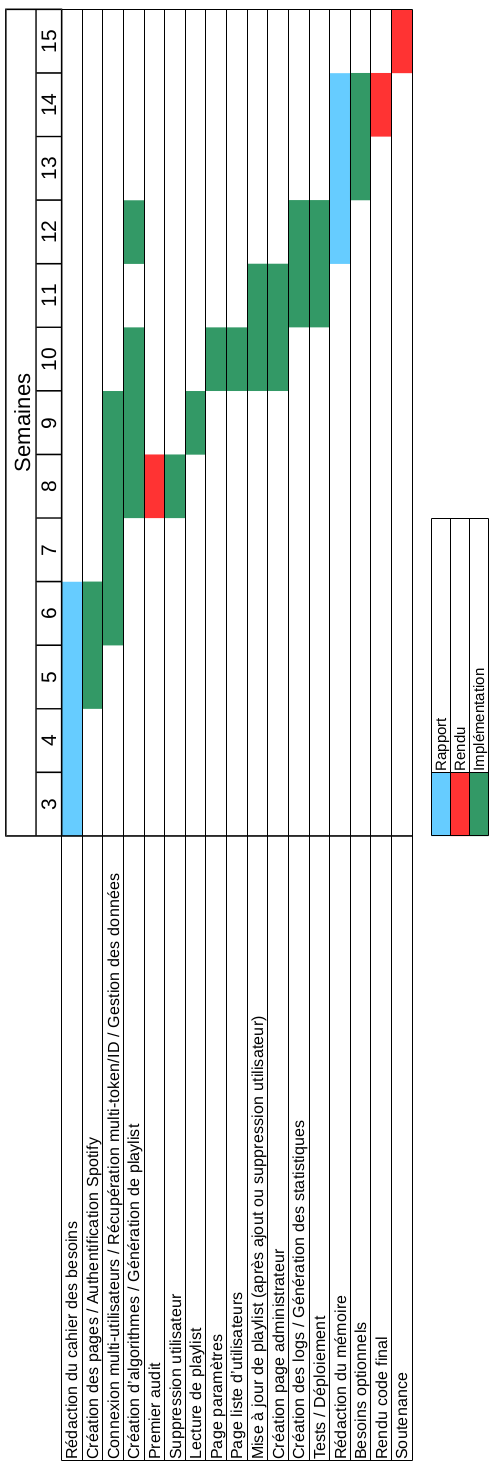
\includegraphics[scale=0.45]{images/gantt.png}

\bibliography{biblio}
\cite{Music}

\end{document}
